\label{sec:Tecniques}

En aquesta secció es descriuen les tècniques de visió per ordinador i tractament d'imatges emprades durant la realització del projecte.

\section{Preprocessat digital d'imatges}
	El preprocessament digital en una imatge, consisteix a aplicar diverses tècniques per tal d'aconseguir una imatge d'on poder obtenir la informació que necessitem més fàcilment. Es tracta
	d'eliminar distorsions o bé ressaltar determinades parts de la imatge.\\\\
	Algunes de les tècniques que es poden aplicar i s'han provat durant la realització del projecte són:

	\begin{itemize}
		\item{\textbf{Suavitzat de la imatge i reducció de soroll:} S'han provat filtres senzills com la mediana.}
		\item{\textbf{Reducció de mides:} Reduir la mida de la imatge ens permet millorar el temps d'execució.}
		\item{\textbf{Escala de grisos:} Els píxels de la imatge passen a tenir un valor en el rang 0-255. D'aquesta manera s'aconsegueix reduir el pes de la imatge. Encara que es perd la informació del color, moltes
		vegades pot ser irrellevant o fins i tot portar a errors.}
		\item{\textbf{Equalització de l'histograma:} Per tal de millorar el contrast de les imatges, s'ha provat d'utilitzar CLAHE (\textit{Contrast Limited Adaptive Histogram Equalization}).}
		\item{\textbf{Operacions morfològiques:} Erode, dilate, open, close}
	\end{itemize}
\noindent
	Finalment, s'ha decidit no aplicar cap filtre i utilitzar les imatges tal com són, ja que o bé no feien cap efecte o funcionaven correctament només amb determinats tipus d'imatges i empitjoraven d'altres.
	El que sí que s'ha fet és reduir la mida i convertir les imatges a escala de grisos.

\newpage
\section{Obtenció de \textit{keypoints} en una imatge}
	Consisteix a obtenir punts de la imatge amb característiques distintives, que ens puguin ser útils més endavant.\\
	\begin{figure}[H]
		\centering
		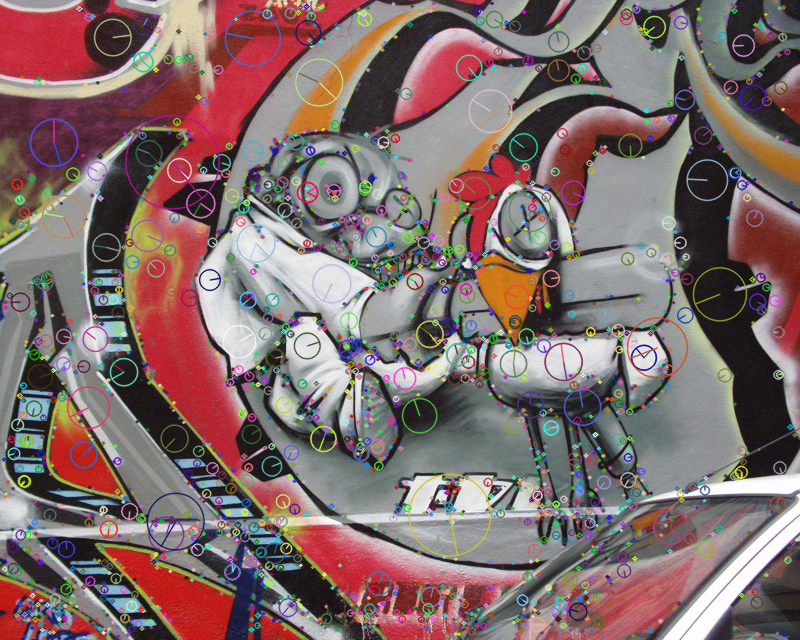
\includegraphics[width=0.65\textwidth]{images/RobotKp}
		\caption{\textit{Keypoints}}
	\end{figure}
	\noindent
	La detecció es pot classificar en:\\
	\begin{itemize}
		\item{Detecció de vores}
		\item{Detecció de cantonades}
		\item{Detecció de regions\\}
	\end{itemize}
	Les principals tècniques d'obtenció de \textit{keypoints} que s'han utilitzat són: SIFT, Harris i ORB.
	També s'han provat altres algorismes com FAST\cite{Rosten:2006:MLH:2094437.2094478}, SURF, MSER\cite{BMVC.16.36:abbreviated} o Shi-Tomasi\cite{Shi:1993:GFT:866676}.

	\subsubsection{Harris}
	Harris és un detector que es basa a trobar cantonades. La idea bàsica és que mitjançant una finestra de NxM píxels, es recorre la imatge buscant els punts on hi ha canvis d'intensitat
	en diverses direccions.\\\\
	Segons els canvis d'intensitat de cada píxel, es poden classificar els punts en \textit{flat}, vores i cantonades.\\\\
	\begin{figure}[H]
		\centering
		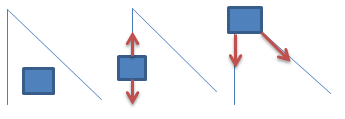
\includegraphics[width=0.7\textwidth]{images/harris}
		\captionsource{\textit{Flat}, vora i cantonada}{Wikipedia}
	\end{figure}
	\noindent
	El problema principal de Harris és que no és invariant a l'escala. Com podeu veure en la figura \ref{fig:vores}, punts considerats cantonades en una escala,
	podrien convertir-se en vores en una altra. Per això, existeixen algunes solucions alternatives com Harris-Laplace.\\\\

	\begin{figure}[H]
		\centering
		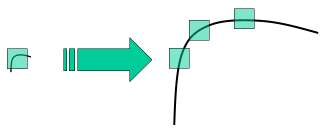
\includegraphics[width=0.6\textwidth]{images/scale_invariant}
		\captionsource{\textit{Vores a diferent escala}}{OpenCV}
		\label{fig:vores}
	\end{figure}
	\noindent
	En el nostre cas, s'ha optat per aplicar Harris en diverses escales, fent una piràmide de la imatge original.

	\subsubsection{SIFT}
	Localització multi-escala mitjançant una diferència de gaussianes (DoG), que s'utilitza com a aproximació d'una laplaciana de gaussianes.\\\\
	{TO-DO}
	DoG s'obté com la diferencia de gaussian blurring de la imatge amb diferents *. Aquest procés es realitza per diferents octaves de la imatge en la
	piràmide gaussiana, tal com es veu en la imatge següent:\\
	\begin{figure}[H]
		\centering
		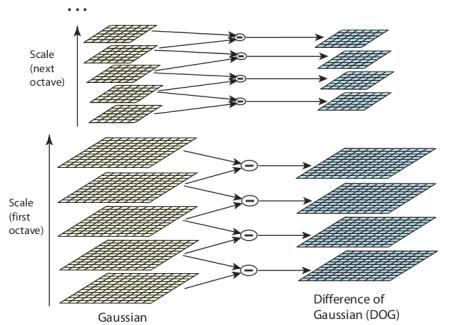
\includegraphics[width=0.7\textwidth]{images/sift_dog}
		\captionsource{\textit{SIFT - DoG}}{OpenCV}
	\end{figure}
	\noindent
	Un cop tenim les DoG, es busquen {local extrema} en l'espai i l'escala. Per cada píxel, es compara amb els seus 8 veïns, així com els 9 píxels de la
	següent escala i els 9 de les anteriors. Si és {local extrema} el considerem potencial \textit{keypoint}.\\
	\begin{figure}[H]
		\centering
		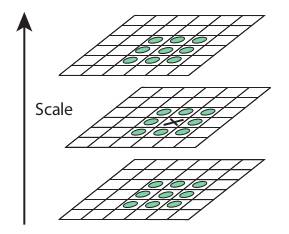
\includegraphics[width=0.4\textwidth]{images/sift_local_extrema}
		\captionsource{\textit{SIFT - Local extrema}}{OpenCV}
	\end{figure}
	\noindent
	Un cop obtinguts els possibles \textit{keypoints}, s'eliminen els menys robustos. S'utilitza [Taylor] per aconseguir una millor localització del [extrema],
	i si la seva intensitat és menor a un llindar (0.03 segons Lowe) es rebutja. També s'han d'eliminar vores, utilitzant un mètode similar a Harris.
	S'agafa una matriu hessiana de 2x2 per calcular la principal corbatura. Sabent que les vores tenen un eigen-value major a l'altre, si la ratio dels
	{eigen-values} supera un llindar (10 per Lowe) es descarta el punt. \\\\
	SIFT també assigna una orientació als punts d'interés per aconseguir ser invariant a la rotació. S'agafa un veinatge al voltant de la localització del
	\textit{keypoint} segons l'escala i es calcula la magnitud i direcció del gradient. Es crea un histograma d'orientació de 36 \textit{bins}
	que cobreix els 360 graus.

	\subsubsection{ORB}
	El detector d'ORB (\textit{Oriented FAST and Rotated BRIEF}) utilitza el detector FAST amb modificacions per millorar el rendiment.\\\\
	FAST és un detector de cantonades enfocat a aconseguir els punts de manera molt ràpida, a canvi d'empitjorar una mica l'eficàcia. S'agafa la intensitat d'un píxel i es compara amb el conjunt
	de N píxels veïns que el rodegen.\\\\
	\begin{figure}[H]
		\centering
		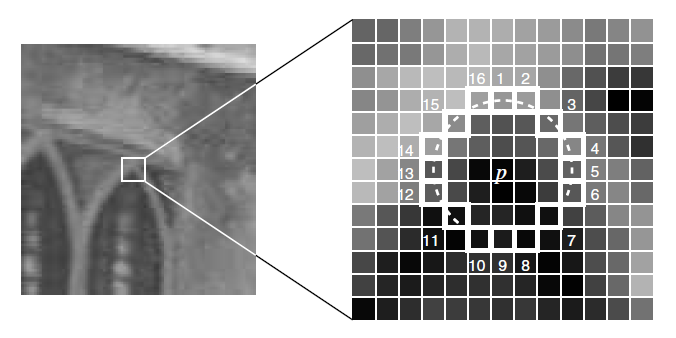
\includegraphics[width=0.55\textwidth]{images/fast}
		\captionsource{FAST, N=16}{-}
	\end{figure}
	\noindent
	Suposant que N = 16 i definint un llindar t, si 12 píxels veïns (\sfrac{3}{4} parts) són majors a I\textsubscript{p} + t o bé menors a I\textsubscript{p} - t, es considera que el punt és d'interès.
	El problema principal de FAST és que no té en compte l'orientació.\\\\
	ORB utilitza FAST aplicant les següents millores:\\
	\begin{itemize}
		\item{S'agafen els N millors punts després d'aplicar la mesura de Harris.}
		\item{Es fa una piràmide per fer multi-escala.}
		\item{S'utilitzen els moments per calcular l'orientació.}
	\end{itemize}

\section{Extracció de característiques}

	L'extracció de característiques és el que ens permetrà comparar els punts obtinguts en les dues imatges.\\
	\begin{itemize}
		\item{Descriptors vectorials: SIFT, SURF}
		\item{Descriptors binaris: ORB, BRISK\\}
	\end{itemize}
	Principalment s'han utilitzat SIFT, ORB i BRISK, encara que també s'han provat d'altres com SURF, LATCH o DAISY\cite{Tola10}.

	\subsubsection{SIFT}
	Per cada \textit{keypoint}, s'agafa un veinatge de 16x16 píxels al voltant del punt. Això es divideix en 16 blocs de mida 4x4. Per cada sub-block,
	es calcula l'histograma d'orientacions en 8 direccions, de manera que podem obtenir 128 valors, que es representaran en forma de vector.\\\\
	A part d'aquest procés, s'apliccaran també mesures per fer més robust el descriptor contra canvis d'intensitat, rotació, etc.
	\begin{figure}[H]
		\centering
		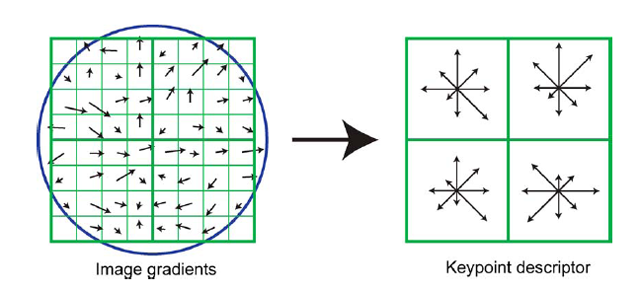
\includegraphics[width=0.65\textwidth]{images/sift-des}
		\captionsource{Descriptor SIFT}{-}
	\end{figure}

	\subsubsection{ORB}
	El descriptor d'ORB és una modificació de BRIEF\cite{Calonder:2010:BBR:1888089.1888148}, un descriptor ràpid i senzill basat en \textit{strings} binaris.\\\\
	Per cada \textit{keypoint} s'agafen N punts veïns i d'aquests s'agafen parells de forma més o menys aleatòria. Per cada parell es compara la intensitat i es retorna un \textit{string} binari de mida N amb '1' o '0' segons
	si la intensitat del primer punt és major a la del segon o no. Això ens permet comparar els descriptors amb una simple operació XOR.\\\\
	És un mètode molt ràpid, però no és invariable ni a la rotació ni a l'escala. Per això, ORB intenta solucionar el problema de la rotació girant els patrons en funció de l'angle de la característica.

	\subsubsection{BRISK}
	És un descriptor binari que utilitza un patró de cercles concèntrics. S'agafen N punts del patró i per cada parell de punts es compara la intensitat del primer amb el segon. Si el valor del primer és
	major, es posa '1', si no '0'.\\\\
	D'aquesta manera s'obté una cadena de N caràcters (binari) molt fàcil de comparar a l'hora de fer \textit{matching}. Utilitzant el mateix patró i seqüència de parells, només caldrà
	comparar les cadenes binàries amb la suma del resultat d'una XOR.
	\begin{figure}[H]
		\centering
		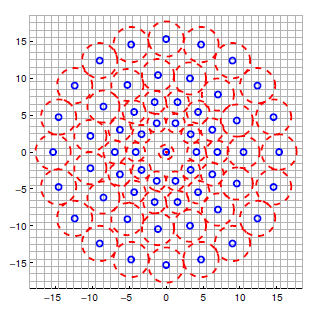
\includegraphics[width=0.5\textwidth]{images/brisk}
		\captionsource{\textit{Sampling pattern} BRISK}{-}
	\end{figure}

%\newpage
\section{\textit{Matching} de característiques}

	Un cop tenim els \textit{keypoints} i les característiques dels punts, necessitarem obtenir coincidències entre els punts de les dues imatges.\\\\
	Bàsicament podem obtenir els aparellaments de dues maneres:\\
	\begin{itemize}	
		\item{Força bruta: Consisteix a provar totes les combinacions possibles per cada punt.}
		\item{Aproximació\\}
	\end{itemize}
	Com que el temps d'execució no és un factor essencial, s'aplicarà el mètode de força bruta, una mica més lent. Pels descriptors binaris s'utilitzarà la distància de Hamming, mentre que pels vectorials
	s'utilitzarà l'euclidiana.\\

	\begin{figure}[H]
		\centering
		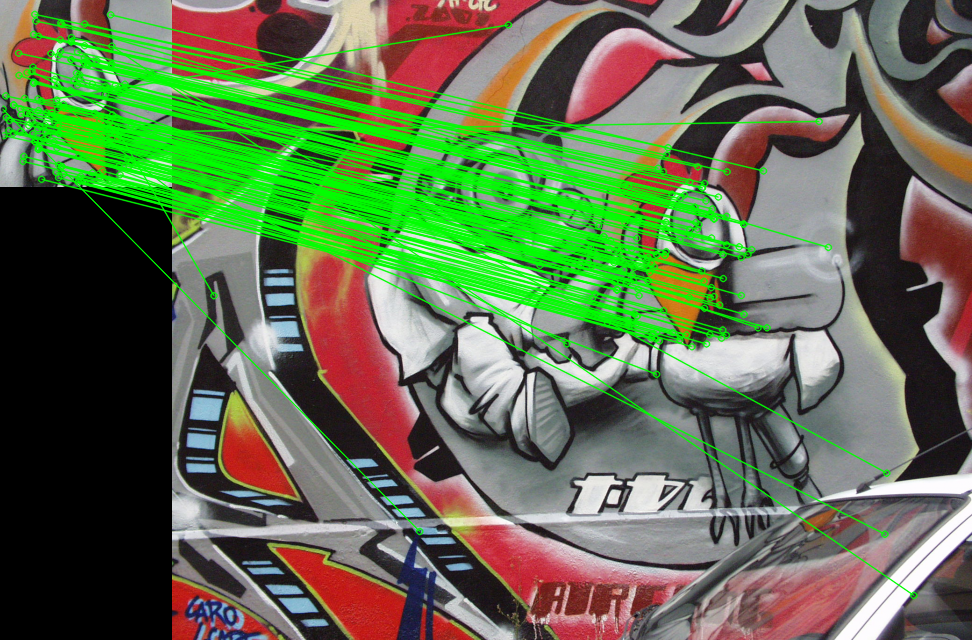
\includegraphics[width=0.7\textwidth]{images/matching}
		\caption{\textit{Matching}}
	\end{figure}
\noindent
	En la imatge anterior podem veure determinats punts on el \textit{match} és clarament erroni. Aquest error es pot minimitzar escollint punts més significatius, característiques més distintives, aplicant
	la ràtio de Lowe o eliminant \textit{outliers}.

%\newpage
\section{Homografia}

	L'objectiu principal del programa és trobar una part d'una imatge en una altra imatge diferent i per fer això utilitzarem l'homografia. Trobant la relació entre els píxels de les dues imatges podrem
	reprojectar el pla d'una imatge en l'altre i trobar el punt on volem dirigir el robot.\\
	\begin{figure}[H]
		\centering
		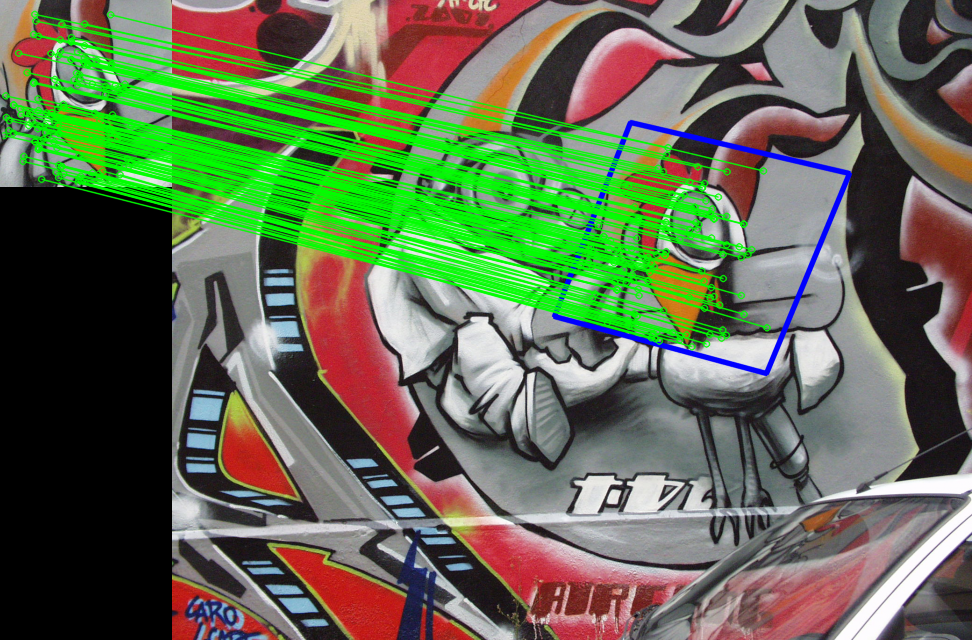
\includegraphics[width=0.7\textwidth]{images/homography}
		\caption{Homografia}
	\end{figure}
	\noindent
	A l'hora de buscar l'homografia aplicarem RANSAC (\textit{Random Sample Consensus})\cite{Fischler:1981:RSC:358669.358692}, un algorisme que ens permetrà eliminar \textit{outliers} dels \textit{match} trobats.\\
	\begin{figure}[H]
		\centering
		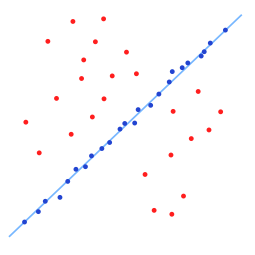
\includegraphics[width=0.45\textwidth]{images/ransac}
		\captionsource{RANSAC}{Wikipedia}
	\end{figure}
